\usepackage[utf8x]{inputenc}
\usepackage[T1]{fontenc}
\usepackage{tikz}
\usepackage{xcolor}

\title{Basic test talk}
\author{François Gindraud\inst{1}}
\institute{\inst{1}Home}
\date{\today}

\newcommand{\Depth}{2}
\newcommand{\Height}{2}
\newcommand{\Width}{2}

\begin{document}

\section*{Title}
\frame{\titlepage}
\section*{Outline}
\frame{\tableofcontents}

\section{Without transitions}
\begin{frame}{Text slide}
	\begin{itemize}
		\item Ein...
		\item Zwei.
		\item Drei !
	\end{itemize}
	\Note{A shiny itemize !}
	\begin{block}{A block !}
		You can put stuff inside ! Its awesome !
	\end{block}
	\Note{Wow... a block !}
	Some text !
	\Note{And a piece of plain text to finish}
\end{frame}

\begin{frame}{Graphic slide}
	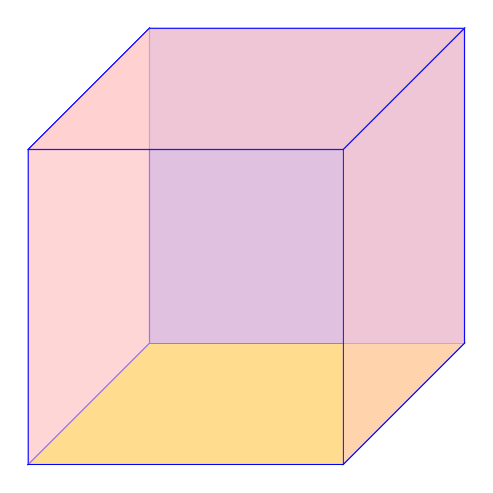
\begin{tikzpicture}[scale=2]
		\coordinate (O) at (0,0,0);
		\coordinate (A) at (0,\Width,0);
		\coordinate (B) at (0,\Width,\Height);
		\coordinate (C) at (0,0,\Height);
		\coordinate (D) at (\Depth,0,0);
		\coordinate (E) at (\Depth,\Width,0);
		\coordinate (F) at (\Depth,\Width,\Height);
		\coordinate (G) at (\Depth,0,\Height);

		\draw[blue,fill=yellow!80] (O) -- (C) -- (G) -- (D) -- cycle;% Bottom Face
		\draw[blue,fill=blue!30] (O) -- (A) -- (E) -- (D) -- cycle;% Back Face
		\draw[blue,fill=red!10] (O) -- (A) -- (B) -- (C) -- cycle;% Left Face
		\draw[blue,fill=red!20,opacity=0.8] (D) -- (E) -- (F) -- (G) -- cycle;% Right Face
		\draw[blue,fill=red!20,opacity=0.6] (C) -- (B) -- (F) -- (G) -- cycle;% Front Face
		\draw[blue,fill=red!20,opacity=0.8] (A) -- (B) -- (F) -- (E) -- cycle;% Top Face
	\end{tikzpicture}
\end{frame}

\section{With transitions}
\begin{frame}{Text slide 2}
	\begin{itemize}[<+->]
		\item Ein...
		\item Zwei.
		\item Drei !
	\end{itemize}
	\Note<.->{A shiny itemize !}
	\begin{block}<+->{A block !}
		You can put stuff inside ! Its awesome !
	\end{block}
	\Note<.->{Wow... a block !}
	\onslide<+->{Some text !}
	\Note<.->{And a piece of plain text to finish}
\end{frame}

\begin{frame}{Graphic slide 2}
	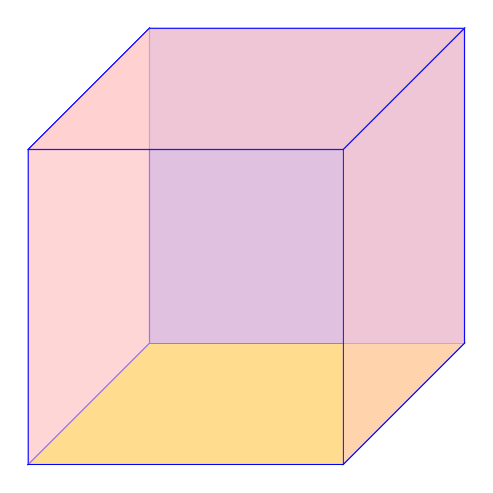
\begin{tikzpicture}[scale=2]
		\coordinate (O) at (0,0,0);
		\coordinate (A) at (0,\Width,0);
		\coordinate (B) at (0,\Width,\Height);
		\coordinate (C) at (0,0,\Height);
		\coordinate (D) at (\Depth,0,0);
		\coordinate (E) at (\Depth,\Width,0);
		\coordinate (F) at (\Depth,\Width,\Height);
		\coordinate (G) at (\Depth,0,\Height);

		\draw<+->[blue,fill=yellow!80] (O) -- (C) -- (G) -- (D) -- cycle;% Bottom Face
		\draw<+->[blue,fill=blue!30] (O) -- (A) -- (E) -- (D) -- cycle;% Back Face
		\draw<+->[blue,fill=red!10] (O) -- (A) -- (B) -- (C) -- cycle;% Left Face
		\draw<+->[blue,fill=red!20,opacity=0.8] (D) -- (E) -- (F) -- (G) -- cycle;% Right Face
		\draw<+->[blue,fill=red!20,opacity=0.6] (C) -- (B) -- (F) -- (G) -- cycle;% Front Face
		\draw<+->[blue,fill=red!20,opacity=0.8] (A) -- (B) -- (F) -- (E) -- cycle;% Top Face
	\end{tikzpicture}
\end{frame}

\section*{Conclusion}
\begin{frame}{End}
	This is the end...
\end{frame}

\end{document}
